%
% MCS.T411 - Computational Complexity
% Author: Hoang Nguyen
%
\documentclass[12pt,twoside]{article}

\usepackage{graphicx}
\usepackage{amsmath}
\usepackage{dsfont}

% Cross-references for handout numbers.

% Updated to include SMA course for Fall 2001 -- cel

\newcommand{\name}{Hoang Nguyen - 15M54097}


\usepackage{latexsym}
%\usepackage{bbm}
\usepackage{times,url}
%\usepackage{clrscode3e}

\newcommand{\mitst}[1]{\begin{description}
\item[MIT students:] #1
\end{description}}
\newcommand{\smast}[1]{\begin{description}
\item[SMA students:] #1
\end{description}}

\newcommand{\profs}{Professors: Nitta, Inoue, and Shinoda}
\newcommand{\subj}{ART.T548}

\newlength{\toppush}
\setlength{\toppush}{2\headheight}
\addtolength{\toppush}{\headsep}

\newcommand{\htitle}[2]{\noindent\vspace*{-\toppush}\newline\parbox{6.5in}
{\textit{Advanced Artificial Intelligence: Spring 2016}\hfill\name\newline
Tokyo Institute of Technology \hfill #2\newline
\profs\hfill #1 \vspace*{-.5ex}\newline
\mbox{}\hrulefill\mbox{}}\vspace*{1ex}\mbox{}\newline
\begin{center}{\Large\bf #1}\end{center}}

\newcommand{\handout}[2]{\thispagestyle{empty}
 \markboth{#1}{#1}
 \pagestyle{myheadings}\htitle{#1}{#2}}

\newcommand{\htitlewithouttitle}[2]{\noindent\vspace*{-\toppush}\newline\parbox{6.5in}
{\textit{Advanced Artificial Intelligence}\hfill#2\newline
Tokyo Institute of Technology \hfill ART.T548\newline
%Singapore-MIT Alliance \hfill SMA5503\newline
\profs\hfill Handout #1\vspace*{-.5ex}\newline
\mbox{}\hrulefill\mbox{}}\vspace*{1ex}\mbox{}\newline}

\newcommand{\handoutwithouttitle}[2]{\thispagestyle{empty}
 \markboth{Handout \protect\ref{#1}}{Handout \protect\ref{#1}}
 \pagestyle{myheadings}\htitlewithouttitle{\protect\ref{#1}}{#2}}

\newcommand{\exam}[2]{% parameters: exam name, date
 \thispagestyle{empty}
 \markboth{\subj\ #1\hspace{1in}Name\hrulefill\ \ }%
          {\subj\ #1\hspace{1in}Name\hrulefill\ \ }
 \pagestyle{myheadings}\examtitle{#1}{#2}
 \renewcommand{\theproblem}{Problem \arabic{problemnum}}
}
\newcommand{\examsolutions}[3]{% parameters: handout, exam name, date
 \thispagestyle{empty}
 \markboth{Handout \protect\ref{#1}: #2}{Handout \protect\ref{#1}: #2}
% \pagestyle{myheadings}\htitle{\protect\ref{#1}}{#2}{#3}
 \pagestyle{myheadings}\examsolutionstitle{\protect\ref{#1}} {#2}{#3}
 \renewcommand{\theproblem}{Problem \arabic{problemnum}}
}
\newcommand{\examsolutionstitle}[3]{\noindent\vspace*{-\toppush}\newline\parbox{6.5in}
{\textit{Advanced Artificial Intelligence}\hfill#3\newline
Tokyo Institute of Technology \hfill ART.T548\newline
%Singapore-MIT Alliance \hfill SMA5503\newline
\profs\hfill Handout #1\vspace*{-.5ex}\newline
\mbox{}\hrulefill\mbox{}}\vspace*{1ex}\mbox{}\newline
\begin{center}{\Large\bf #2}\end{center}}

\newcommand{\takehomeexam}[2]{% parameters: exam name, date
 \thispagestyle{empty}
 \markboth{\subj\ #1\hfill}{\subj\ #1\hfill}
 \pagestyle{myheadings}\examtitle{#1}{#2}
 \renewcommand{\theproblem}{Problem \arabic{problemnum}}
}

\makeatletter
\newcommand{\exambooklet}[2]{% parameters: exam name, date
 \thispagestyle{empty}
 \markboth{\subj\ #1}{\subj\ #1}
 \pagestyle{myheadings}\examtitle{#1}{#2}
 \renewcommand{\theproblem}{Problem \arabic{problemnum}}
 \renewcommand{\problem}{\newpage
 \item \let\@currentlabel=\theproblem
 \markboth{\subj\ #1, \theproblem}{\subj\ #1, \theproblem}}
}
\makeatother


\newcommand{\examtitle}[2]{\noindent\vspace*{-\toppush}\newline\parbox{6.5in}
{\textit{Advanced Artificial Intelligence}\hfill#2\newline
Tokyo Institute of Technology \hfill ART.T548 Sprint 2016\newline
%Singapore-MIT Alliance \hfill SMA5503\newline
\profs\hfill #1\vspace*{-.5ex}\newline
\mbox{}\hrulefill\mbox{}}\vspace*{1ex}\mbox{}\newline
\begin{center}{\Large\bf #1}\end{center}}

\newcommand{\grader}[1]{\hspace{1cm}\textsf{\textbf{#1}}\hspace{1cm}}

\newcommand{\points}[1]{[#1 points]\ }
\newcommand{\parts}[1]
{
  \ifnum#1=1
  (1 part)
  \else
  (#1 parts)
  \fi
  \ 
}

\newcommand{\bparts}{\begin{problemparts}}
\newcommand{\eparts}{\end{problemparts}}
\newcommand{\ppart}{\problempart}

%\newcommand{\lg} {lg\ }

\setlength{\oddsidemargin}{0pt}
\setlength{\evensidemargin}{0pt}
\setlength{\textwidth}{6.5in}
\setlength{\topmargin}{0in}
\setlength{\textheight}{8.5in}


\renewcommand{\cases}[1]{\left\{ \begin{array}{ll}#1\end{array}\right.}
\newcommand{\cif}[1]{\mbox{if $#1$}}
\newcommand{\cwhen}[1]{\mbox{when $#1$}}

\newcounter{problemnum}
\newcommand{\theproblem}{Problem \theproblemsetnum-\arabic{problemnum}}
\newenvironment{problems}{
        \begin{list}{{\bf \theproblem. \hspace*{0.5em}}}
        {\setlength{\leftmargin}{0em}
         \setlength{\rightmargin}{0em}
         \setlength{\labelwidth}{0em}
         \setlength{\labelsep}{0em}
         \usecounter{problemnum}}}{\end{list}}
\makeatletter
\newcommand{\problem}[1][{}]{\item \let\@currentlabel=\theproblem \textbf{#1}}
\makeatother

\newcounter{problempartnum}[problemnum]
\newenvironment{problemparts}{
        \begin{list}{{\bf (\alph{problempartnum})}}
        {\setlength{\leftmargin}{2.5em}
         \setlength{\rightmargin}{2.5em}
         \setlength{\labelsep}{0.5em}}}{\end{list}}
\newcommand{\problempart}{\addtocounter{problempartnum}{1}\item}

\newenvironment{truefalseproblemparts}{
        \begin{list}{{\bf (\alph{problempartnum})\ \ \ T\ \ F\hfil}}
        {\setlength{\leftmargin}{4.5em}
         \setlength{\rightmargin}{2.5em}
         \setlength{\labelsep}{0.5em}
         \setlength{\labelwidth}{4.5em}}}{\end{list}}

\newcounter{exercisenum}
\newcommand{\theexercise}{Exercise \theproblemsetnum-\arabic{exercisenum}}
\newenvironment{exercises}{
        \begin{list}{{\bf \theexercise. \hspace*{0.5em}}}
        {\setlength{\leftmargin}{0em}
         \setlength{\rightmargin}{0em}
         \setlength{\labelwidth}{0em}
         \setlength{\labelsep}{0em}
        \usecounter{exercisenum}}}{\end{list}}
\makeatletter
\newcommand{\exercise}{\item \let\@currentlabel=\theexercise}
\makeatother

\newcounter{exercisepartnum}[exercisenum]
%\newcommand{\problem}[1]{\medskip\mbox{}\newline\noindent{\bf Problem #1.}\hspace*{1em}}
%\newcommand{\exercise}[1]{\medskip\mbox{}\newline\noindent{\bf Exercise #1.}\hspace*{1em}}

\newenvironment{exerciseparts}{
        \begin{list}{{\bf (\alph{exercisepartnum})}}
        {\setlength{\leftmargin}{2.5em}
         \setlength{\rightmargin}{2.5em}
         \setlength{\labelsep}{0.5em}}}{\end{list}}
\newcommand{\exercisepart}{\addtocounter{exercisepartnum}{1}\item}


% Macros to make captions print with small type and 'Figure xx' in bold.
\makeatletter
\def\fnum@figure{{\bf Figure \thefigure}}
\def\fnum@table{{\bf Table \thetable}}
\let\@mycaption\caption
%\long\def\@mycaption#1[#2]#3{\addcontentsline{\csname
%  ext@#1\endcsname}{#1}{\protect\numberline{\csname 
%  the#1\endcsname}{\ignorespaces #2}}\par
%  \begingroup
%    \@parboxrestore
%    \small
%    \@makecaption{\csname fnum@#1\endcsname}{\ignorespaces #3}\par
%  \endgroup}
%\def\mycaption{\refstepcounter\@captype \@dblarg{\@mycaption\@captype}}
%\makeatother
\let\mycaption\caption
%\newcommand{\figcaption}[1]{\mycaption[]{#1}}

\newcounter{totalcaptions}
\newcounter{totalart}

\newcommand{\figcaption}[1]{\addtocounter{totalcaptions}{1}\caption[]{#1}}

% \psfigures determines what to do for figures:
%       0 means just leave vertical space
%       1 means put a vertical rule and the figure name
%       2 means insert the PostScript version of the figure
%       3 means put the figure name flush left or right
\newcommand{\psfigures}{0}
\newcommand{\spacefigures}{\renewcommand{\psfigures}{0}}
\newcommand{\rulefigures}{\renewcommand{\psfigures}{1}}
\newcommand{\macfigures}{\renewcommand{\psfigures}{2}}
\newcommand{\namefigures}{\renewcommand{\psfigures}{3}}

\newcommand{\figpart}[1]{{\bf (#1)}\nolinebreak[2]\relax}
\newcommand{\figparts}[2]{{\bf (#1)--(#2)}\nolinebreak[2]\relax}


\macfigures     % STATE

% When calling \figspace, make sure to leave a blank line afterward!!
% \widefigspace is for figures that are more than 28pc wide.
\newlength{\halffigspace} \newlength{\wholefigspace}
\newlength{\figruleheight} \newlength{\figgap}
\newcommand{\setfiglengths}{\ifnum\psfigures=1\setlength{\figruleheight}{\hruleheight}\setlength{\figgap}{1em}\else\setlength{\figruleheight}{0pt}\setlength{\figgap}{0em}\fi}
\newcommand{\figspace}[2]{\ifnum\psfigures=0\leavefigspace{#1}\else%
\setfiglengths%
\setlength{\wholefigspace}{#1}\setlength{\halffigspace}{.5\wholefigspace}%
\rule[-\halffigspace]{\figruleheight}{\wholefigspace}\hspace{\figgap}#2\fi}
\newlength{\widefigspacewidth}
% Make \widefigspace put the figure flush right on the text page.
\newcommand{\widefigspace}[2]{
\ifnum\psfigures=0\leavefigspace{#1}\else%
\setfiglengths%
\setlength{\widefigspacewidth}{28pc}%
\addtolength{\widefigspacewidth}{-\figruleheight}%
\setlength{\wholefigspace}{#1}\setlength{\halffigspace}{.5\wholefigspace}%
\makebox[\widefigspacewidth][r]{#2\hspace{\figgap}}\rule[-\halffigspace]{\figruleheight}{\wholefigspace}\fi}
\newcommand{\leavefigspace}[1]{\setlength{\wholefigspace}{#1}\setlength{\halffigspace}{.5\wholefigspace}\rule[-\halffigspace]{0em}{\wholefigspace}}

% Commands for including figures with macpsfig.
% To use these commands, documentstyle ``macpsfig'' must be specified.
\newlength{\macfigfill}
\makeatother
\newlength{\bbx}
\newlength{\bby}
\newcommand{\macfigure}[5]{\addtocounter{totalart}{1}
\ifnum\psfigures=2%
\setlength{\bbx}{#2}\addtolength{\bbx}{#4}%
\setlength{\bby}{#3}\addtolength{\bby}{#5}%
\begin{flushleft}
\ifdim#4>28pc\setlength{\macfigfill}{#4}\addtolength{\macfigfill}{-28pc}\hspace*{-\macfigfill}\fi%
\mbox{\psfig{figure=./#1.ps,%
bbllx=#2,bblly=#3,bburx=\bbx,bbury=\bby}}
\end{flushleft}%
\else\ifdim#4>28pc\widefigspace{#5}{#1}\else\figspace{#5}{#1}\fi\fi}
\makeatletter

\newlength{\savearraycolsep}
\newcommand{\narrowarray}[1]{\setlength{\savearraycolsep}{\arraycolsep}\setlength{\arraycolsep}{#1\arraycolsep}}
\newcommand{\normalarray}{\setlength{\arraycolsep}{\savearraycolsep}}

\newcommand{\hint}{{\em Hint:\ }}

% Macros from /th/u/clr/mac.tex

\newcommand{\set}[1]{\left\{ #1 \right\}}
\newcommand{\abs}[1]{\left| #1\right|}
\newcommand{\card}[1]{\left| #1\right|}
\newcommand{\floor}[1]{\left\lfloor #1 \right\rfloor}
\newcommand{\ceil}[1]{\left\lceil #1 \right\rceil}
\newcommand{\ang}[1]{\ifmmode{\left\langle #1 \right\rangle}
   \else{$\left\langle${#1}$\right\rangle$}\fi}
        % the \if allows use outside mathmode,
        % but will swallow following space there!
\newcommand{\paren}[1]{\left( #1 \right)}
\newcommand{\bracket}[1]{\left[ #1 \right]}
\newcommand{\prob}[1]{\Pr\left\{ #1 \right\}}
\newcommand{\Var}{\mathop{\rm Var}\nolimits}
\newcommand{\expect}[1]{{\rm E}\left[ #1 \right]}
\newcommand{\expectsq}[1]{{\rm E}^2\left[ #1 \right]}
\newcommand{\variance}[1]{{\rm Var}\left[ #1 \right]}
\renewcommand{\choose}[2]{{{#1}\atopwithdelims(){#2}}}
\def\pmod#1{\allowbreak\mkern12mu({\rm mod}\,\,#1)}
\newcommand{\matx}[2]{\left(\begin{array}{*{#1}{c}}#2\end{array}\right)}
\newcommand{\Adj}{\mathop{\rm Adj}\nolimits}

\newtheorem{theorem}{Theorem}
\newtheorem{lemma}[theorem]{Lemma}
\newtheorem{corollary}[theorem]{Corollary}
\newtheorem{xample}{Example}
\newtheorem{definition}{Definition}
\newenvironment{example}{\begin{xample}\rm}{\end{xample}}
\newcommand{\proof}{\noindent{\em Proof.}\hspace{1em}}
\def\squarebox#1{\hbox to #1{\hfill\vbox to #1{\vfill}}}
\newcommand{\qedbox}{\vbox{\hrule\hbox{\vrule\squarebox{.667em}\vrule}\hrule}}
\newcommand{\qed}{\nopagebreak\mbox{}\hfill\qedbox\smallskip}
\newcommand{\eqnref}[1]{(\protect\ref{#1})}

%%\newcommand{\twodots}{\mathinner{\ldotp\ldotp}}
\newcommand{\transpose}{^{\mbox{\scriptsize \sf T}}}
\newcommand{\amortized}[1]{\widehat{#1}}

\newcommand{\punt}[1]{}

%%% command for putting definitions into boldface
% New style for defined terms, as of 2/23/88, redefined by THC.
\newcommand{\defn}[1]{{\boldmath\textit{\textbf{#1}}}}
\newcommand{\defi}[1]{{\textit{\textbf{#1\/}}}}

\newcommand{\red}{\leq_{\rm P}}
\newcommand{\lang}[1]{%
\ifmmode\mathord{\mathcode`-="702D\rm#1\mathcode`\-="2200}\else{\rm#1}\fi}

%\newcommand{\ckt}[1]{\ifmmode\mathord{\mathcode`-="702D\sc #1\mathcode`\-="2200}\else$\mathord{\mathcode`-="702D\sc #1\mathcode`\-="2200}$\fi}
\newcommand{\ckt}[1]{\ifmmode \sc #1\else$\sc #1$\fi}

%% Margin notes - use \notesfalse to turn off notes.
\setlength{\marginparwidth}{0.6in}
\reversemarginpar
\newif\ifnotes
\notestrue
\newcommand{\longnote}[1]{
  \ifnotes
    {\medskip\noindent Note: \marginpar[\hfill$\Longrightarrow$]
      {$\Longleftarrow$}{#1}\medskip}
  \fi}
\newcommand{\note}[1]{
  \ifnotes
    {\marginpar{\tiny \raggedright{#1}}}
  \fi}


\newcommand{\reals}{\mathbbm{R}}
\newcommand{\integers}{\mathbbm{Z}}
\newcommand{\naturals}{\mathbbm{N}}
\newcommand{\rationals}{\mathbbm{Q}}
\newcommand{\complex}{\mathbbm{C}}

\newcommand{\oldreals}{{\bf R}}
\newcommand{\oldintegers}{{\bf Z}}
\newcommand{\oldnaturals}{{\bf N}}
\newcommand{\oldrationals}{{\bf Q}}
\newcommand{\oldcomplex}{{\bf C}}

\newcommand{\w}{\omega}                 %% for fft chapter

\newenvironment{closeitemize}{\begin{list}
{$\bullet$}
{\setlength{\itemsep}{-0.2\baselineskip}
\setlength{\topsep}{0.2\baselineskip}
\setlength{\parskip}{0pt}}}
{\end{list}}

% These are necessary within a {problems} environment in order to restore
% the default separation between bullets and items.
\newenvironment{normalitemize}{\setlength{\labelsep}{0.5em}\begin{itemize}}
                              {\end{itemize}}
\newenvironment{normalenumerate}{\setlength{\labelsep}{0.5em}\begin{enumerate}}
                                {\end{enumerate}}

%\def\eqref#1{Equation~(\ref{eq:#1})}
%\newcommand{\eqref}[1]{Equation (\ref{eq:#1})}
\newcommand{\eqreftwo}[2]{Equations (\ref{eq:#1}) and~(\ref{eq:#2})}
\newcommand{\ineqref}[1]{Inequality~(\ref{ineq:#1})}
\newcommand{\ineqreftwo}[2]{Inequalities (\ref{ineq:#1}) and~(\ref{ineq:#2})}

\newcommand{\figref}[1]{Figure~\ref{fig:#1}}
\newcommand{\figreftwo}[2]{Figures \ref{fig:#1} and~\ref{fig:#2}}

\newcommand{\liref}[1]{line~\ref{li:#1}}
\newcommand{\Liref}[1]{Line~\ref{li:#1}}
\newcommand{\lirefs}[2]{lines \ref{li:#1}--\ref{li:#2}}
\newcommand{\Lirefs}[2]{Lines \ref{li:#1}--\ref{li:#2}}
\newcommand{\lireftwo}[2]{lines \ref{li:#1} and~\ref{li:#2}}
\newcommand{\lirefthree}[3]{lines \ref{li:#1}, \ref{li:#2}, and~\ref{li:#3}}

\newcommand{\lemlabel}[1]{\label{lem:#1}}
\newcommand{\lemref}[1]{Lemma~\ref{lem:#1}} 

\newcommand{\exref}[1]{Exercise~\ref{ex:#1}}

\newcommand{\handref}[1]{Handout~\ref{#1}}

\newcommand{\defref}[1]{Definition~\ref{def:#1}}

% (1997.8.16: Victor Luchangco)
% Modified \hlabel to only get date and to use handouts counter for number.
%   New \handout and \handoutwithouttitle commands in newmac.tex use this.
%   The date is referenced by <label>-date.
%   (Retained old definition as \hlabelold.)
%   Defined \hforcelabel to use an argument instead of the handouts counter.

\newcounter{handouts}
\setcounter{handouts}{0}

\newcommand{\hlabel}[2]{%
\stepcounter{handouts}
{\edef\next{\write\@auxout{\string\newlabel{#1}{{\arabic{handouts}}{0}}}}\next}
\write\@auxout{\string\newlabel{#1-date}{{#2}{0}}}
}

\newcommand{\hforcelabel}[3]{%          Does not step handouts counter.
\write\@auxout{\string\newlabel{#1}{{#2}{0}}}
\write\@auxout{\string\newlabel{#1-date}{{#3}{0}}}}


% less ugly underscore
% --juang, 2008 oct 05
\renewcommand{\_}{\vrule height 0 pt depth 0.4 pt width 0.5 em \,}


\setlength{\oddsidemargin}{0pt}
\setlength{\evensidemargin}{0pt}
\setlength{\textwidth}{6.5in}
\setlength{\topmargin}{0in}
\setlength{\textheight}{8.5in}

% Fill these in!
\newcommand{\theproblemsetnum}{1}
\newcommand{\releasedate}{September 29, 2016~~}
\newcommand{\partaduedate}{Tuesday,  15}
\newcommand{\tabUnit}{3ex}
\newcommand{\tabT}{\hspace*{\tabUnit}}

\begin{document}

\handout{Assignment \theproblemsetnum}{\releasedate}

\newif\ifsolution
\solutiontrue
\newcommand{\solution}{\textbf{Solution:}}

Analyze \texttt{weather.nominal.arff} using Weka \texttt{3.6.14}

\setlength{\parindent}{0pt}

\medskip

\hrulefill

\textbf{Collaborators:}
%%% COLLABORATORS START %%%
None.
%%% COLLABORATORS END %%%

\begin{exercises}

\problem \textbf{Compute posterior distribution for the class}

Use NaiveBayesSimple to find a Bayesian classifier (Laplace estimator = 1 
is used in order to avoid frequency problems). Compute P(``yes'') and 
P(``no'') of the following instances.

\begin{exerciseparts}
  \exercisepart Windy = True

  \ifsolution \solution{}
    Given the evidence Windy = True, with independence assumption
    and Bayes rule, we have the probability of answer ``yes'' as:
    \begin{equation*}
      \begin{aligned}
        \mbox{P}(\mbox{``yes''} | \mbox{Windy = True}) & = 
        \frac{\mbox{P}(\mbox{Windy = True} | \mbox{``yes''}) \times
        \mbox{P}(\mbox{``yes''})}{\mbox{P}(\mbox{Windy = True})}
      \end{aligned}
    \end{equation*}
    Because of the independence assumption between attributes, 
    we have the prior for Windy = True as follow:
    \begin{equation*}
      \begin{aligned}
        \mbox{P}(\mbox{Windy = True}) 
          = \ & \mbox{P}(\mbox{Windy = True}|\mbox{``yes''})  \times \mbox{P}(\mbox{``yes''})\ \ + \\
            & \mbox{P}(\mbox{Windy = True}|\mbox{``no''})  \times \mbox{P}(\mbox{``no''}) \\
          = \ & 0.3636 \times 0.625 + 0.5714 \times 0.375 \\
          = \ & 0.4415
      \end{aligned}
    \end{equation*}
    We have the posterior distribution for the class given Windy = True:
    \begin{equation*}
      \begin{aligned}
        \mbox{P}(\mbox{``yes''} | \mbox{Windy = True}) 
        = & \ \frac{\mbox{P}(\mbox{Windy = True} | \mbox{``yes''}) \times
        \mbox{P}(\mbox{``yes''})}{\mbox{P}(\mbox{Windy = True})} \\
        = & \ \frac{0.3636 \times 0.625}{0.4415} \\
        = & \ \boldsymbol{0.5} \\
        \mbox{P}(\mbox{``no''} | \mbox{Windy = True}) 
        = & \ 1 - \mbox{P}(\mbox{``yes''} | \mbox{Windy = True})  \\
        = & \ \boldsymbol{0.5}
      \end{aligned}
    \end{equation*}
  \fi

  \exercisepart Humidity = High, Windy = True

  \ifsolution \solution{}
    Similar to question 1-(a), we have the join prior probability
    for the case Humidity = High (abbr. H = High), Windy = True
    (abbr. W = True) as follow:
    \begin{equation*}
      \begin{aligned}
        \mbox{P}(\mbox{H = High, W = True}) 
          = \ & \mbox{P}(\mbox{H = High, W = True}|\mbox{``yes''})  \times \mbox{P}(\mbox{``yes''})\ \ + \\
            & \mbox{P}(\mbox{H = High, W = True}|\mbox{``no''})  \times \mbox{P}(\mbox{``no''})
      \end{aligned}
    \end{equation*}
    Apply the attribute independence assumption, we have the following
    fractorization of the conditional join probability:
    \begin{equation*}
      \begin{aligned}
        \mbox{P}(\mbox{H = High, W = True}) 
          = \ & \mbox{P}(\mbox{H = High}|\mbox{``yes''}) \times 
                \mbox{P}(\mbox{W = True}|\mbox{``yes''}) \times \mbox{P}(\mbox{``yes''})\ \ + \\
              & \mbox{P}(\mbox{H = High}|\mbox{``no''}) \times
                \mbox{P}(\mbox{W = True}|\mbox{``no''}) \times \mbox{P}(\mbox{``no''}) \\
          = \ & 0.3636 \times 0.3636 \times 0.625 + 0.5714 \times 0.7142 \times 0.375 \\
          = \ & 0.2357
      \end{aligned}
    \end{equation*}
    We have the posterior distribution for the class given Windy = True and Humidity = High:
    \begin{equation*}
      \begin{aligned}
        \mbox{P}(\mbox{``yes''} | \mbox{H = High, W = True}) 
        = & \ \frac{\mbox{P}(\mbox{W = True, H = High} | \mbox{``yes''}) \times
        \mbox{P}(\mbox{``yes''})}{\mbox{P}(\mbox{H = High, W = True})} \\
        = & \ \frac{0.3636 \times 0.3636 \times 0.625}{0.2357} \\
        = & \ \boldsymbol{0.35} \\
        \mbox{P}(\mbox{``no''} | \mbox{H = High, W = True}) 
        = & \ 1 - \mbox{P}(\mbox{``yes''} | \mbox{H = High, Windy = True})  \\
        = & \ \boldsymbol{0.65}
      \end{aligned}
    \end{equation*}
  \fi 

  \exercisepart Temperature = Hot, Humidity = High, Windy = True

  \ifsolution \solution{}
    Similar to question 1-(a,b), we have the join prior probability
    for the case Temperature = Hot (abbr. T = Hot) Humidity = High 
    (abbr. H = High), Windy = True (abbr. W = True) as follow:
    \begin{equation*}
      \begin{aligned}
        \mbox{P}(\mbox{T = Hot, H = High, W = True}) 
          = \ & \mbox{P}(\mbox{T = Hot, H = High, W = True}|\mbox{``yes''})  \times \mbox{P}(\mbox{``yes''})
          \\ & + \ 
             \mbox{P}(\mbox{T = Hot, H = High, W = True}|\mbox{``no''})  \times \mbox{P}(\mbox{``no''})
      \end{aligned}
    \end{equation*}
    Apply the attribute independence assumption, we have the following
    fractorization of the conditional join probability:
    \begin{equation*}
      \begin{aligned}
        \mbox{P}(\mbox{T = Hot, H = High, W = True}) 
          = \ & \mbox{P}(\mbox{T = Hot}|\mbox{``yes''}) \times
                \mbox{P}(\mbox{H = High}|\mbox{``yes''}) \times \\
              & \ \ \ \mbox{P}(\mbox{W = True}|\mbox{``yes''}) \times \mbox{P}(\mbox{``yes''})\ \ + \\
              & \mbox{P}(\mbox{T = Hot}|\mbox{``no''}) \times
                \mbox{P}(\mbox{H = High}|\mbox{``no''}) \times \\
              & \ \ \ \mbox{P}(\mbox{W = True}|\mbox{``no''}) \mbox{P}(\mbox{``no''}) \\
          = \ & 0.25 \times 0.3636 \times 0.3636 \times 0.625 + 
              0.375 \times 0.5714 \times 0.7142 \times 0.375 \\
          = \ & 0.078
      \end{aligned}
    \end{equation*}
    We have the posterior distribution for the class given Temperature = Hot, Windy = True, and Humidity = High:
    \begin{equation*}
      \begin{aligned}
        \mbox{P}(\mbox{``yes''} | \mbox{T = Hot, H = High, W = True}) 
        = & \ \frac{\mbox{P}(\mbox{T = Hot, W = True, H = High} | \mbox{``yes''}) \times
        \mbox{P}(\mbox{``yes''})}{\mbox{P}(\mbox{T = Hot, H = High, W = True})} \\
        = & \ \frac{0.25 \times 0.3636 \times 0.3636 \times 0.625}{0.078} \\
        = & \ \boldsymbol{0.26} \\
        \mbox{P}(\mbox{``no''} | \mbox{T = Hot, H = High, W = True}) 
        = & \ 1 - \mbox{P}(\mbox{``yes''} | \mbox{T = Hot, H = High, Windy = True})  \\
        = & \ \boldsymbol{0.74}
      \end{aligned}
    \end{equation*}
  \fi
\end{exerciseparts}

\problem \textbf{J48 decision tree}

\begin{exerciseparts}

\exercisepart 
Use J48 to find a decision tree.

\ifsolution \solution{}
The decision tree found by J48 with defaut setting is:
\begin{figure}[h]
  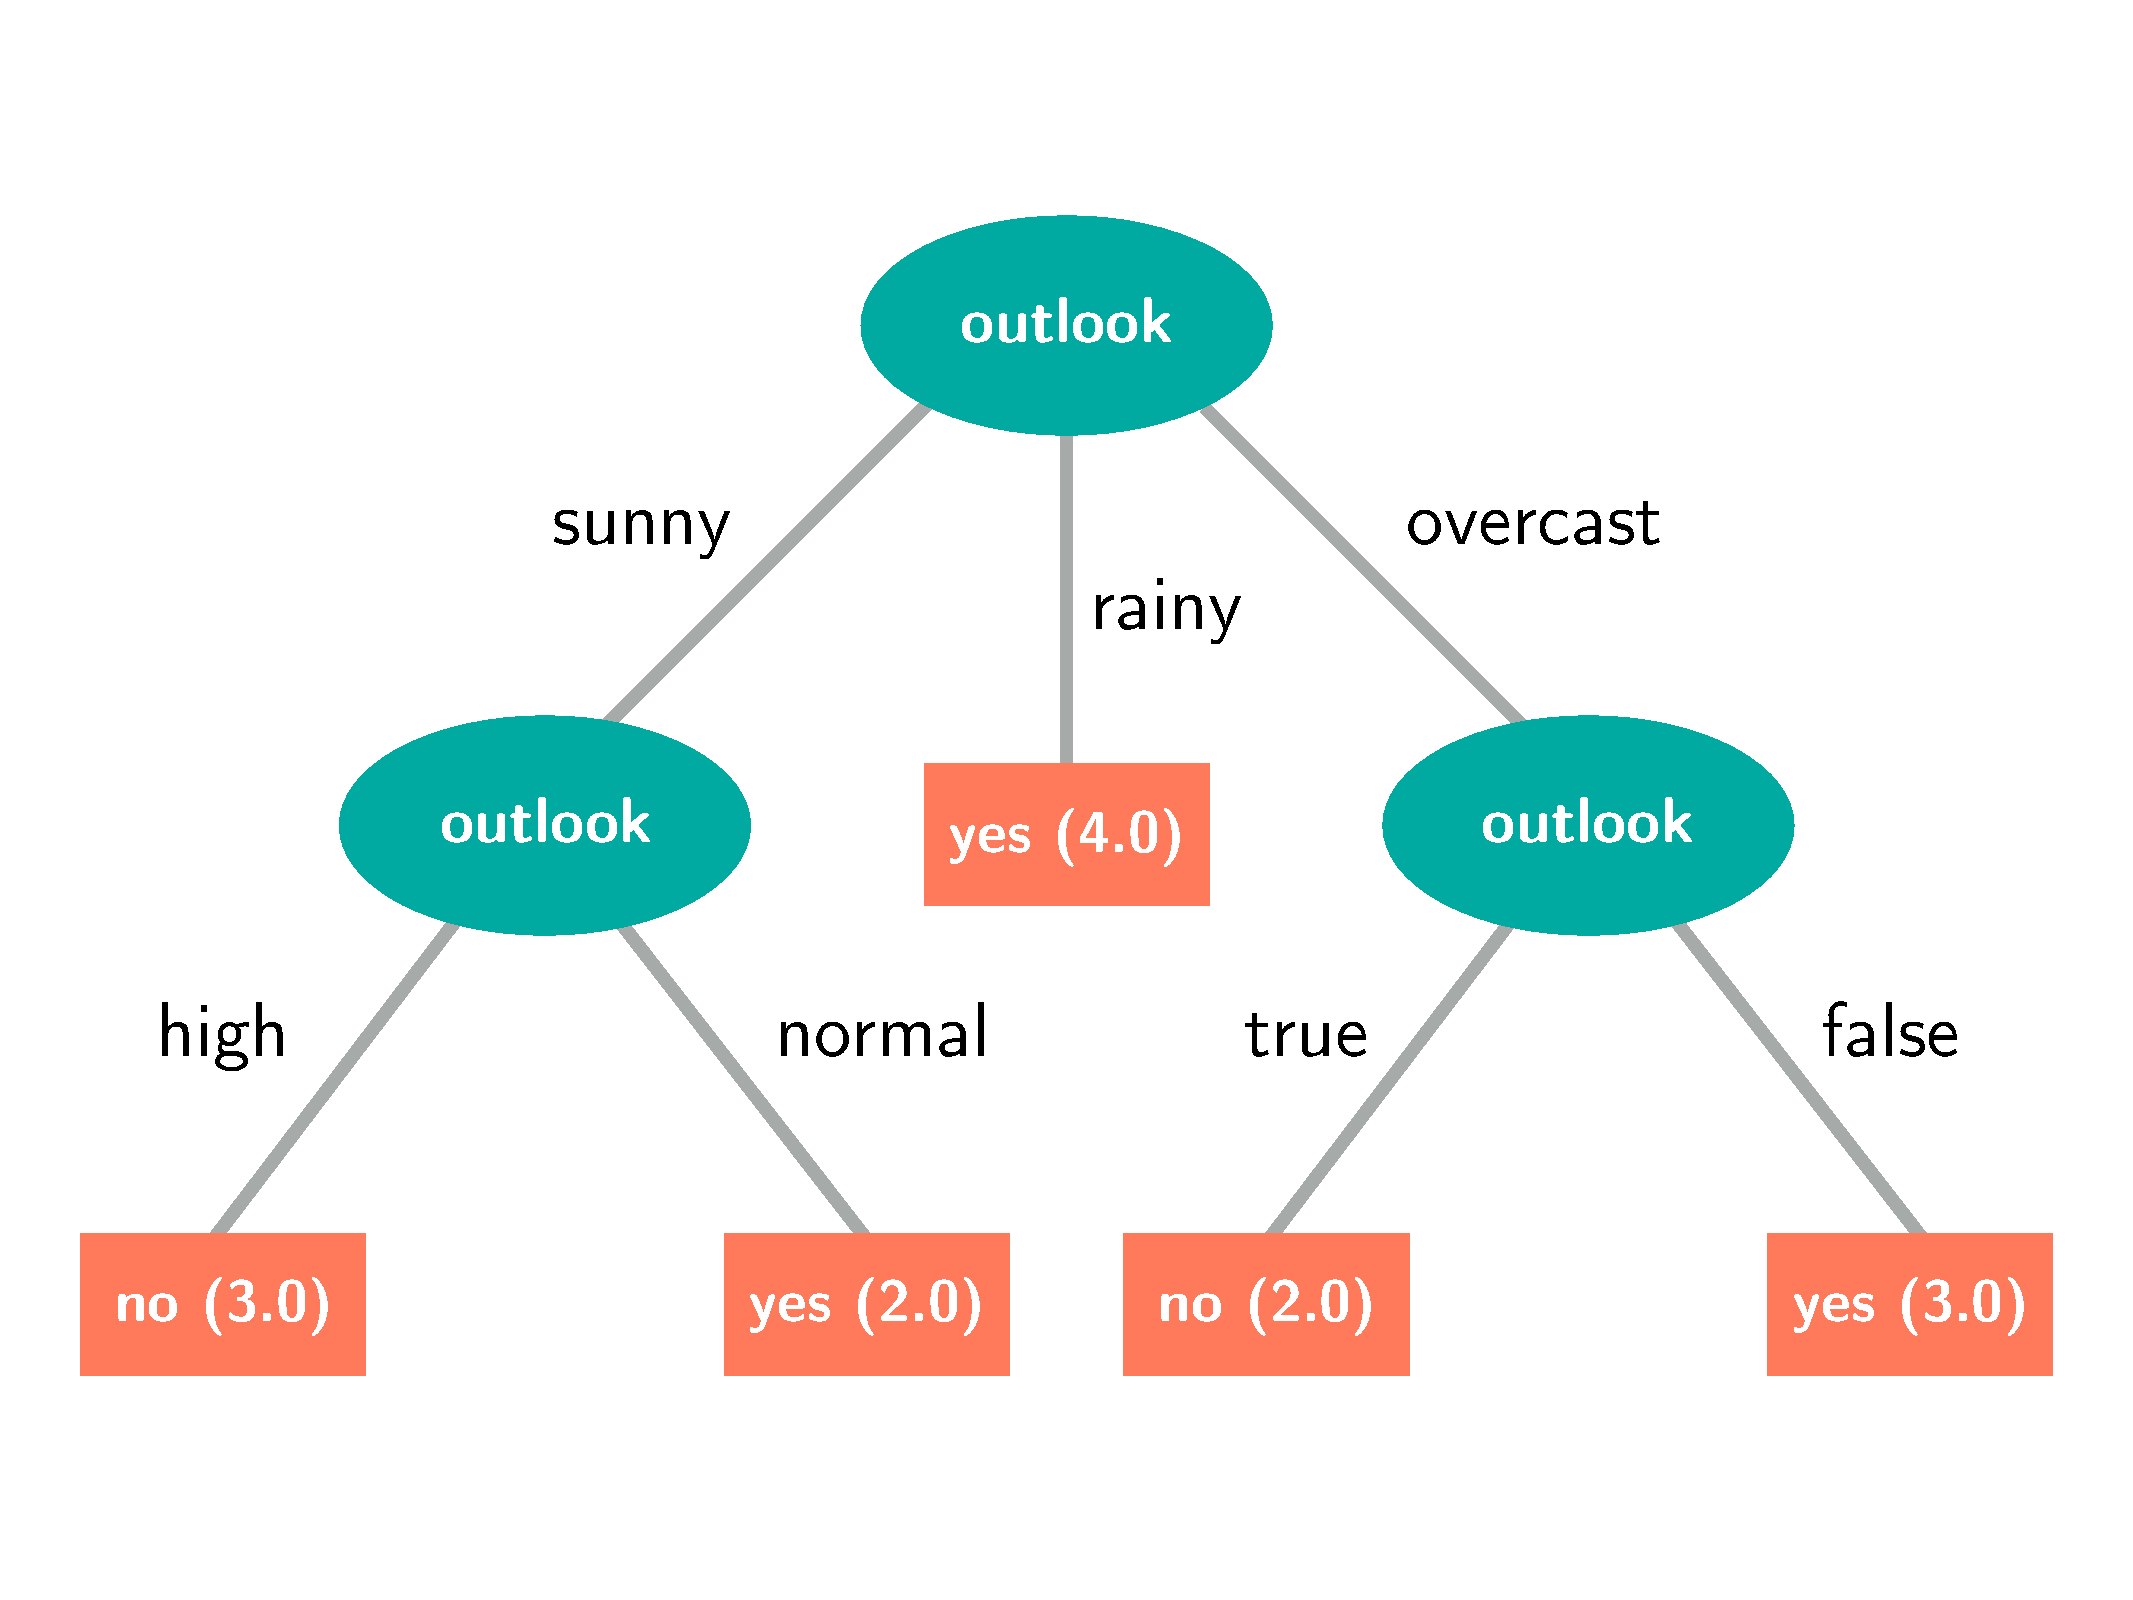
\includegraphics[width=0.8\textwidth]{j48tree.pdf}
  \centering
\end{figure}
\fi

\exercisepart
Check its accuracy to the original data by hand.

\ifsolution \solution{}
The accuracy of the tree over the training data is \textbf{100\%}.
This result is due to the tree is created by using full
dataset. However, the accuracy of the tree is only 50\% if
checked with 10-fold cross-validation.
\fi

\exercisepart
Why is ``\texttt{outlook}'' selected as its root attribute? 
Compare with other attribute (temperature, humidity and windy)
and answer quantitatively.

\ifsolution \solution{}
``\texttt{outlook}'' is selected as its root attribute because its
information gain is the largest out of all attributes. We can compute
the expected information of each attribute as follow:
\begin{equation*}
  \begin{aligned}
    \mathds{E} \ [\mathcal{I} (\mbox{Outlook})] & = \mbox{info}([2,3],[4,0],[3,2]) = 0.693 \\
    \mathds{E} \ [\mathcal{I} (\mbox{Temperature})] & = \mbox{info}([3,1],[2,2],[4,2]) = 0.911 \\
    \mathds{E} \ [\mathcal{I} (\mbox{Humidity})] & = \mbox{info}([6,1],[3,4]) = 0.788 \\
    \mathds{E} \ [\mathcal{I} (\mbox{Windy})] & = \mbox{info}([6,2],[3,3]) = 0.892 \\
  \end{aligned}
\end{equation*}
Infomation gain for each attribute: 
\begin{equation*}
  \begin{aligned}
    \mathds{G} (\mbox{Outlook}) & = \mbox{info}([9,5]) - 0.693 = 0.247 \\
    \mathds{G} (\mbox{Temperature}) & = \mbox{info}([9,5]) - 0.911 = 0.029 \\
    \mathds{G} (\mbox{Humidity}) & = \mbox{info}([9,5]) - 0.788 = 0.152 \\
    \mathds{G} (\mbox{Windy}) & = \mbox{info}([9,5]) - 0.892 = 0.048 \\
  \end{aligned}
\end{equation*}
Attribute \textbf{outlook} gives the largest information gain. 
Therefore it is selected as the root attribute.
\fi

\end{exerciseparts}

\problem \textbf{Use Prism to find rules}

\begin{exerciseparts}

\exercisepart
Show all rules.

\ifsolution \solution{}
The rules derived from Prism algorithm: \\
\texttt{=== Classifier model (full training set)} \\
\texttt{Prism rules} \\
\texttt{-----------} \\
\texttt{If outlook = overcast then yes} \\
\texttt{If humidity = normal} \\
\texttt{~~~and windy = FALSE then yes} \\
\texttt{If temperature = mild} \\
\texttt{~~~and humidity = normal then yes} \\
\texttt{If outlook = rainy} \\
\texttt{~~~and windy = FALSE then yes} \\
\texttt{If outlook = sunny} \\
\texttt{~~~and humidity = high then no} \\
\texttt{if outlook = rainy} \\
\texttt{~~~and windy = TRUE then no} \\
\texttt{Time taken to build model: 0.01 seconds}
\fi

\exercisepart
Check the accuracy (confidence) and the converage
(support) of each rule to the original data by hand.

\ifsolution \solution{}
\begin{itemize}
  \item \texttt{If outlook = overcast then yes}: Support = 4; accuracy = 100\%.
  \item \texttt{If humidity = normal and windy = FALSE then yes}: Support = 4; accuracy = 100\%.
  \item \texttt{If temperature = mild and humidity = normal then yes}: Support = 2; accuracy = 100\%.
  \item \texttt{If outlook = rainy and windy = FALSE then yes}: Support = 3; accuracy = 100\%.
  \item \texttt{If outlook = sunny and humidity = high then o}: Support = 3; accuracy = 100\%.
  \item \texttt{If outlook = rainy and windy = TRUE then no}: Support = 2; accuracy = 100\%.
\end{itemize}
\fi

\exercisepart
Compare (i) the above rules and (ii) rules coverted from the above
decision tree. Is there any instance that is not covered by the 
rules (i) or rules (ii)?

\ifsolution \solution{}
There is a slight difference between (i) and (ii) is there is
two rules in set (i) are replaced by a single rule in set (i).
\texttt{If humidity = normal and windy = FALSE then yes} \\
\texttt{If temperature = mild and humidity = normal then yes} \\
is replaced by:
\texttt{If outlook = sunny and humidity = normal then yes} \\

Checking by hand we can see that both rule sets covered the
dataset. There is no instance that is not covered.
\fi
\end{exerciseparts}
\end{exercises}
\end{document}
